\documentclass{article} % What kind of document this is
\usepackage{tikz} % Import the tikz package
\usetikzlibrary{automata,positioning,arrows}

\tikzset{node distance=2.5cm, % Minimum distance between two nodes. Change if necessary.
  every state/.style={ % Sets the properties for each state
    semithick,
    fill=gray!10},
  initial text={},
  double distance=2pt,
  every edge/.style={
    draw,
    ->,>=stealth,
    semithick}}
\let\epsilon\varepsilon

\begin{document}
  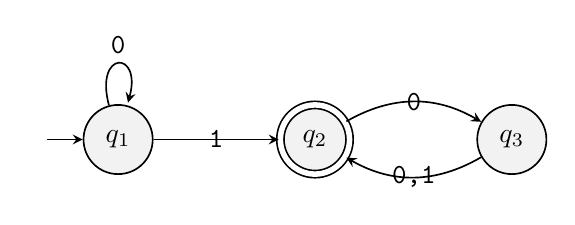
\begin{tikzpicture}
    \node[state,initial](q1){$q_1$};
    \node[state,accepting, right of=q1] (q2) {$q_2$};
    \node[state, right of=q2] (q3) {$q_3$};
    \draw (q1) edge [loop above] node {\tt 0} (q1);
    \draw (q1) edge node {\tt 1} (q2);
    \draw (q2) edge [bend left] node {\tt 0} (q3);
    \draw (q3) edge [bend left] node {\tt 0,1} (q2);
  \end{tikzpicture}

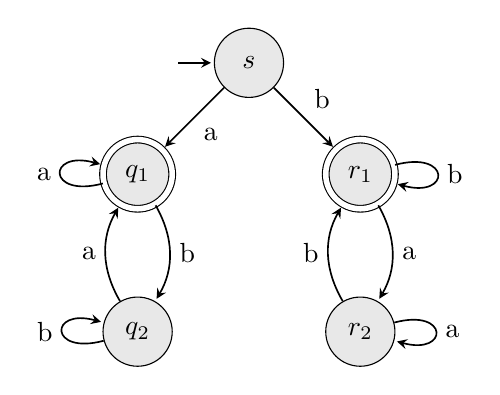
\begin{tikzpicture}[shorten >=1pt,node distance=2cm,auto]
  \tikzstyle{every state}=[fill={rgb:black,1;white,10}]

  \node[state,initial]   (s)                      {$s$};
  \node[state,accepting] (q_1) [below left of=s]  {$q_1$};
  \node[state]           (q_2) [below of=q_1]     {$q_2$};
  \node[state,accepting] (r_1) [below right of=s] {$r_1$};
  \node[state]           (r_2) [below of=r_1]     {$r_2$};

  \path[->]
  (s)   edge              node {a} (q_1)
        edge              node {b} (r_1)
  (q_1) edge [loop left]  node {a} (   )
        edge [bend left]  node {b} (q_2)
  (q_2) edge [loop left]  node {b} (   )
        edge [bend left]  node {a} (q_1)
  (r_1) edge [loop right] node {b} (   )
        edge [bend left]  node {a} (r_2)
  (r_2) edge [loop right] node {a} (   )
        edge [bend left]  node {b} (r_1);
\end{tikzpicture}


\end{document}
